
\section{Dynamic Programming}
\begin{frame}{Rod Cutting Problem}
  Given a rod of length $n$ inches and a table of prices $p_i$
  for $i = 1, 2, ..., n$, determine the maximum revenue $r_n$ obtainable
  by cutting up the rod and selling the pieces.

  \flushright{
    \scriptsize{(Cormen, Thomas H.. Introduction to Algorithms (p. 360). MIT Press).}}
\end{frame}

\begin{frame}
  \begin{tabular}{|c|cccc|cccccc|}\hline
    length $i$  & 1 & 2 & 3 & 4 & 5  & 6  & 7  & 8  & 9  & 10 \\ \hline
    price $p_i$ & 1 & 5 & 8 & 9 & 10 & 17 & 17 & 20 & 24 & 30 \\ \hline
  \end{tabular} \pause

  
  \centering{
    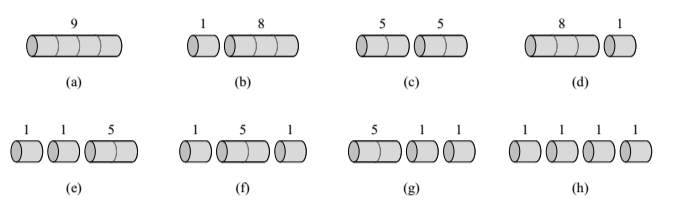
\includegraphics[scale=0.35]{images/rod-cutting}
  }

  \pause

  \begin{itemize}
   \item when $n = 4$, we have $2^{3}$ alternatives for cutting the rod. \pause
   \item $r_4  = max(p_4, r_3 + r_1, r_2 + r_2, r_1 + r_3)$ \pause
   \item $r_n  = max(p_n, r_1 + r_{n-1}, r_2 + r_{n-2}, ..., r_{n-1} + r1)$ \pause
   \item $r_n = max(p_i + r_{n-i})$, for $1 \geq i \geq n$       
  \end{itemize}
\end{frame}

\begin{frame}{Note}

  \begin{itemize}
  \item The {\color{blue}Rod Cutting} problem exhibits
    optimal substructure\pause: optimal solutions
    to a problem incorporate optimal solutions to related subproblems. 
  \end{itemize}
\end{frame}

\begin{frame}{Recursive top-down algorithm}

  \begin{block}{Recursive top-down strategy}
  \begin{algorithmic}
    \Procedure{CutRod}{p, n}
      \If{$n = 0$}
        \State {\bf return} $0$ 
      \EndIf
      \State $q = - \infty$
      \For{$i = 1 .. n$}
         \State $q = max(q, p[i] + CutRod(p, n-i))$ 
         \EndFor
      \State {\bf return} $q$   
    \EndProcedure
  \end{algorithmic}  
  \end{block}

\end{frame}

\begin{frame}[fragile]
  \begin{scriptsize}
  \begin{lstlisting}[language=Java]
public class RecursiveImplementation implements RodCutting {
  private static final int LESS_INFINITE = Integer.MIN_VALUE;

  @Override
  public int cutRod(int[] p, int n) {
    if(n == 0) {
      return 0;
    }
    int q = LESS_INFINITE;
    for(int i = 1; i <= n; i++) {
      q = max(q, p[i] + cutRod(p, n - i));
    }
    return q;
  }
}
  \end{lstlisting}
  \end{scriptsize}
\end{frame}

\begin{frame}
  \begin{itemize}
  \item Ineficient implementation: for $n = 10$, the algorithm
    calls \texttt{CutRod} 1024 times.
  \end{itemize}

  \pause
 
\vskip+1em
 \centering{   
  \begin{scriptsize}
  \begin{tabular}{cc} \toprule
     Value of $n$ & Number of calls \\ \midrule 
     0 & 512 \\
     1 & 256 \\
     2 & 128 \\
     3 & 64 \\
     4 & 32 \\
     5 & 16 \\
     6 & 8 \\
     7 & 4 \\
     8 & 2 \\
     9 & 1 \\
     10 & 1 \\ \bottomrule
  \end{tabular}
  \end{scriptsize}
  }

\end{frame}

\begin{frame}

  \begin{itemize}
  \item Optimization: keep precomputed values in a table (a process named {\color{blue}memoization}). \pause Here we use additional memory to save
    computation time (one of
  the components of dynamic programming).

  \end{itemize}
\end{frame}


\begin{frame}
  \begin{block}{Recursive top-down with memoization}
\begin{small}
    \begin{algorithmic}
      \Procedure{MemoizedCutRod}{p,n}
        \State $r = new Array[0..n]$
        \For{$i = 0 ... n$}
           \State $r[i] = - \infty$
        \EndFor
        \State $CutRodAux(p, n, r)$   
        \EndProcedure
    \end{algorithmic}
    \pause 
    \begin{algorithmic}
      \Procedure{CutRodAux}{p, n, r}
      \If{$r[n] \geq 0$}
        \State {\bf return} $r[n]$
      \EndIf
      \If{$n = 0$}
        \State $q = 0$ 
      \Else
        \State $q = - \infty$
        \For{$i = 1 .. n$}
          \State $q = max(q, p[i] + CutRodAux(p, n-i, r))$ 
        \EndFor
      \EndIf
      \State $r[n] = q$   
      \State {\bf return} $q$   
    \EndProcedure
  \end{algorithmic}  
 \end{small}
  \end{block}
\end{frame}


\begin{frame}
  \begin{block}{Bottom-up with memoization}
\begin{small}
    \begin{algorithmic}
      \Procedure{BottomUpCutRod}{p, n}
      \State $r = new Array[0..n]$
      \State $r[0] = 0$
      \For{$j = 1 ... n$}
       \State $q = - \infty$
       \For{$i = 1 ... j$}
          \State $q = max(q, p[i] + r[j-i]$
          \EndFor
          r[j] = q
       \EndFor
      \State {\bf return} $r[n]$   
    \EndProcedure
  \end{algorithmic}  
 \end{small}
  \end{block}
\end{frame}

\begin{frame}
  Most often, we are not only interested in computing the
  max revenue, but also find the places one must cut the rod to 
  lead to the max revenue. \pause There is a clever extension that adapts the
  bottom up solution to capture the first cut, and then
  reconstruct the entire solution. 
\end{frame}

\begin{frame}
  \begin{small}
    \begin{algorithmic}
      \Procedure{BottomUpCutRod}{p, n}
      \State $r = new Array[0..n]$
      \State $s = new Array[0..n]$

      \State $r[0] = 0$
      \For{$j = 1 ... n$}
       \State $q = - \infty$
       \For{$i = 1 ... j$}
       \If{$q  <  p[i] + r[j-i]$}
         \State $q = p[i] + r[j-i]$
         \State $s[j] = i$ 
       \EndIf
       \EndFor
          r[j] = q
       \EndFor
      \State {\bf return} $r[n], s$   
    \EndProcedure
    \end{algorithmic}
   \end{small} 

\end{frame}


\begin{frame}[fragile]{Longest Common Subsequence Problem}

  \begin{itemize}
  \item Application: compare (part of) the DNA of two (or more)
    different organisms. 
  \end{itemize}
  \pause

\begin{block}{Example} 
\begin{verbatim}
S1 = ACCGGTCGAGTGCGCGGAAGCCGGCCGAA
S2 = GTCGTTCGGAATGCCGTTGCTCTGTAAA
\end{verbatim}
\end{block}
\end{frame}

\begin{frame}
  
\begin{itemize}
\item The similarity between strands S1 and S2 might be
  computed by finding a common, third strand S3 in which the bases in S3 appear
  in each of S1 and S2. Note: the bases must appear  in the same order,
  but not necessarily at the same positions. The longest-common-subsequence is the
  longer common subsequence.

  \pause
  
\item Given two sequences $X = \langle A, B, C, B, D, A, B \rangle$ and
  $Y = \langle B, D, C, A, B, A \rangle$, the sequences $\langle B, C, A \rangle$ and
  $\langle B, C, B, A \rangle$ are common subsequences of both $X$ and $Y$\pause---the
  second one is one of the LCSs. 
\end{itemize}

\flushright{\scriptsize{(Cormen, Thomas H.. Introduction to Algorithms (p. 391). MIT Press.).}}

\end{frame}

\begin{frame}{Optimal Substructure of an LCS}

  Consider two sequences \seqb{X}{x_1, x_2, \ldots, x_m} and \seqb{Y}{y_1, y_2, \ldots, y_n} and
  let \seqb{Z}{z_1, z_2, \ldots, z_k} be any LCS of $X$ and $Y$. As such, one of the following
  situations might happen:

  \begin{small}
  \begin{enumerate}
    \item If $x_m = y_n$, then $z_k = x_m = y_n$ and $z_{k-1}$ is an LCS of $X_{m-1}$ and $Y_{n-1}$.
    \item If $x_m \neq y_n$ and $z_k \neq x_m$, then Z is an LCS of $X_{m-1}$ and $Y$.
    \item If $x_m \neq y_n$ and $z_k \neq x_m$, then Z is an LCS of $X$ and $Y_{n-1}$  
  \end{enumerate}
  \end{small}
\end{frame}

\begin{frame}{A recursive solution}

  \begin{itemize}
  \item Compute $c[i,j]$ as the length of an LCS of the sequences $X_i$ and $Y_j$.
    If either $i = 0$ or $j = 0$, one of the sequences has length $0$, and so the LCS
    has length $0$. \pause
  \end{itemize}
  
\[ 
c[i,j]= \left\{
\begin{array}{ll}
      0                         & if\ i = 0\ or\ j=0 \\ 
      c[i-1,j-1] + 1            & if\ i , j > 0\ and\ x_i = y_j \\   
      max(c[i, j-1], c[i-1,j])  & if\ i , j > 0\ and\ x_i \neq y_j
\end{array} 
\right. 
\]
  
\end{frame}  

\begin{frame}{A dynamic programming algorithm for LCS}

\begin{tiny}
    \begin{algorithmic}
      \Procedure{LCS}{X, Y}
      \State $m = X.length$
      \State $n = Y.length$
      \State $b = Array[1..m, 1..n]$
      \State $c = Array[1..m, 1..n]$
      \For{$i = 1 \ldots m$}
        \State $c[i, 0] = 0$
      \EndFor
      \For{$j = 1 \ldots n$}
        \State $c[0, j] = 0$
      \EndFor
      \For{$i = 1 \ldots m$}
        \For{$j = 1 \ldots n$}
          \If{$X[i] = Y[j]$}
            \State $c[i, j] = c[i-1, j-1] + 1$
            \State $b[i, j] = \nwarrow$
          \ElsIf {$c[i-1, j] \geq c[i, j-1]$}
            \State $c[i, j] = c[i-1, j]$
            \State $b[i, j] = \uparrow$
          \Else
            \State $c[i, j] = c[i, j-1]$
            \State $b[i, j] = \leftarrow$
         \EndIf  
       \EndFor
     \EndFor
      \State {\bf return} $c \ and\ b$    
    \EndProcedure
    \end{algorithmic}
   \end{tiny} 
\end{frame}


\begin{frame}
  \centering{
    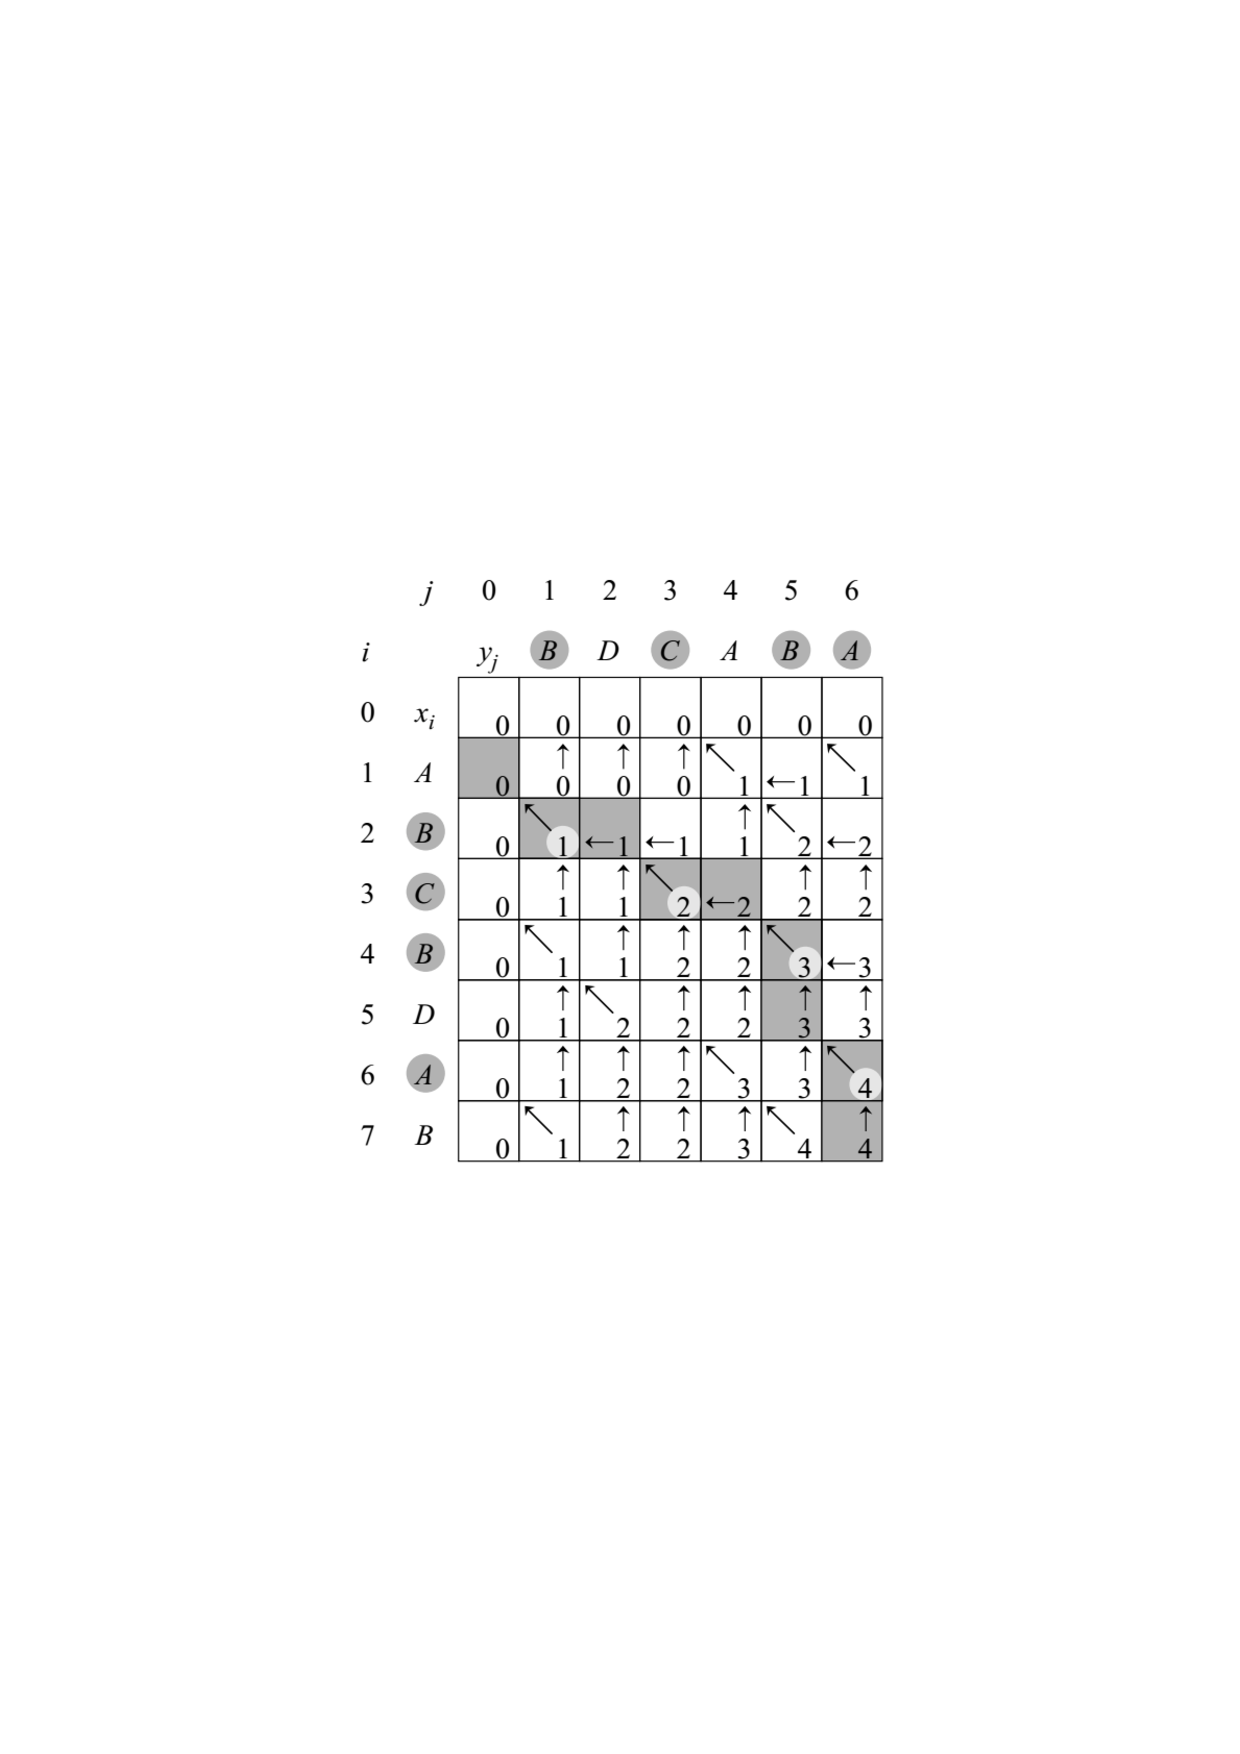
\includegraphics[trim=2cm 2cm 2cm 6cm,scale=0.5]{images/lcs.pdf}
    }
\end{frame}
\begin{frame}
\titlepage
\end{frame}
